\section{Ergebnisse}

In diesem Kapitel wird zunächst das Gesamtergebnis präsentiert. Im Anschluss wird auf Besonderheiten bei Tafel- und Texterkennung eingegangen. Basis der Auswertung ist dabei ein Testdatensatz aus 292 Bildern, worunter sich 79 Bildern mit Tafeln befinden\footnote{Fotos, auf denen die Tafeln nur teilweise zu sehen sind, wurden hier als Fotos ohne Tafeln gewertet.}.
Schließlich werden Versuche mit den Datensätzen anderer Projekte präsentiert.

%Gesamtergebnis mit Genauigkeiten bei Box, Text und insgesamt
\subsection{Gesamtergebnis}
Für das Gesamtergebnis wurden die Tafelausschnitte in den vier Varianten gemeinsam der Texterkennung unterzogen (Vgl. collection.csv). Der durchschnittliche  \textit{F-Score} (\textit{Gesamt}) betrug 0.49. Die Durchschnittswerte der zeilenweisen (\textit{Zeilen}) und buchstabenweisen (\textit{Buchstaben}) Texterkennung lagen bei 0.51 bzw. 0.47. Die durch das Programm als bestes Ergebnis ausgewählten Zeichenketten (\textit{Endauswahl}) erzielten einen \textit{F-Score} von 0.61. Das theoretische Optimum (\textit{Optimum}), also der Durchschnitt der tatsächlichen besten Ergebnisse pro Bild, lag bei 0.7 (Tabelle \ref{tab:Tabelle1}). 19 der insgesamt 412 Tafelausschnitte konnten nicht ausgelesen werden. Daraus resultierte eine nicht ausgelesene Tafel (letztlich eine Falsch-Negative), in den übrigen Fällen konnten die Tafeln über andere Bildausschnitte gelesen werden.
%Das schlechteste Ergebnis wurde bei catacom\_1110 erzielt, auf dem Text nur bei einem von 5 Ausschnitten erkannt wurde (\textit{F-Score} 0.15). Das beste Ergebnis war ein \textit{F-Score} von 1 bei catacom\_1152.\\
\\
\begin{table}
\begin{tabular}[h!]{c|c|c|c|c|c}
Verfahren & Buchstaben & Zeilen & Gesamt & Endauswahl & Optimum \\
\hline
Gesamt & 0.47 & 0.51 & 0.49 & 0.61 & 0.7 \\
Adaptive Hough & 0.43 & 0.47 & 0.45 & 0.49 & 0.56\\
Adaptive Simple & 0.52 & 0.57 & 0.54 & 0.61 & 0.64\\
Iterative Hough & 0.44 & 0.47 & 0.45 & 0.47 & 0.52\\
Iterative Simple & 0.51 & 0.56 & 0.54 & 0.57 & 0.6\\
\end{tabular}
\caption{\label{tab:Tabelle1}Mittelwerte der Ergebnisse bei der Anwendung aller Verfahren gleichzeitig sowie der einzelnen Kombinationen aus Detektions- und Ausschnittverfahren. Angegeben sind die F-Werte für das \textbf{Buchstaben}verfahren (image to box), das \textbf{Zeilen}verfahren (image to text), der \textbf{Gesamt}durchschnitt beider Verfahren, die durch den Algorithmus vorgenommene \textbf{Endauswahl} sowie das theoretische \textbf{Optimum}, also die tatsächliche beste Auswahl.}
\end{table}

\subsection{Tafelerkennung}
%recall, precision und f-score für die Tafelfindung
Bei der Tafelerkennung zeigten  die beiden Kontur-basierten Ansätze gute Ergebnisse, die nur in Nuancen voneinander abwichen.
So erkannte der adaptive Ansatz aus 292 Bildern 133 mit Tafeln. Dass diese Zahl über der der 79 Tafeln lag, ist darin begründet, dass der äußere und der innere Tafelrand als Tafel identifiziert werden können, es also bis zu zwei richtige Erkennungen pro Bild geben kann \footnote{Der Einfluss dieses Umstandes auf die Kennwerte ist so gering, dass er vernachlässigbar ist.}. Zudem wurden 8 Falsch-Positive erkannt, Falsch-Negative gab es keine. Der \textit{Recall} lag damit, wie gewünscht, bei 1. Die \textit{Precision} betrug 0.926, der \textit{F-Score} damit 0.961.
Beim iterativen Ansatz wurden 85 Tafeln erkannt. Da dieser Ansatz nur das wahrscheinlichste Ergebnis pro Bild ausgibt und hier keine Falsch-Negativen auftraten, lag die Zahl der Falsch-Positiven bei 6. Der \textit{Recall} war also auch hier 1, die \textit{Precision} 0.929. Der \textit{F-Score} betrug 0.963.
Die relativ hohe Zahl der Falsch-Positiven resultierte aus vier Fotos, auf denen Plakate abgebildet waren. Da Plakate alle Kriterien der Tafeln erfüllen -- rechteckig, passendes Seitenverhältnis, mit Text beschrieben -- konnte der Algorithmus weder in diesem Schritt noch später, bei der Texterkennung, diese Bilder aussortieren. Eine manuelle Entfernung der Bilder aus dem Datensatz, die sich auch in der Praxis als erster Schritt empfehlen würde, steigerte den \textit{F-Score} auf 0.992 beim adaptiven und auf 0.987 beim iterativen Ansatz. Die Unterschiede zwischen beiden Ansätzen sind also gering, wobei die Anfälligkeit für Falsch-Positive im iterativen Ansatz etwas niedriger ist. 

Weniger erfolgreich verlief die Detektion der Tafeln mit CNNs. Das Grabungsareal entspricht nicht den üblichen in einer Trainingsdatenbank enthaltenen Szenerien. Einzelne Objekte auf dem Gelände, so z.B. Rohrleitungen, der Messstab und der Nordungspfeil, wurden oft als Objekte identifiziert(Abb.\ref{fig:coco}), allerdings mit wechselnder Kategorisierung. Die Tafeln selbst wurden nur in Einzelfällen erkannt, entweder als Schere oder als Sportball (Abb.\ref{fig:cnnboard}. Eine Systematik war nicht festzustellen. Dieser Ansatz muss also als gescheitert betrachtet werden.

\begin{figure}[h!]
\centering
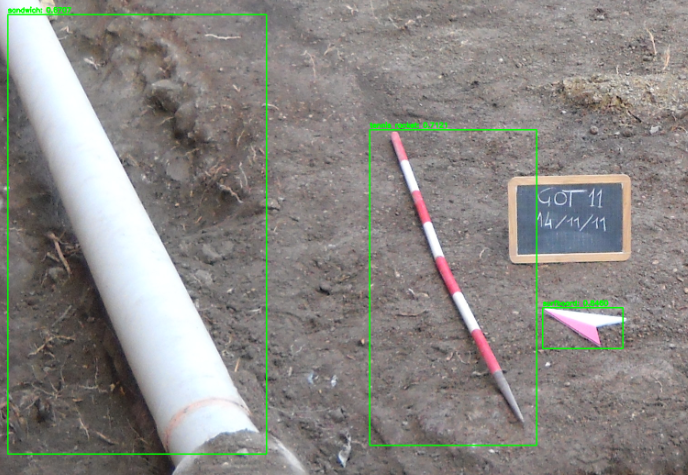
\includegraphics[width =0.5\textwidth]{coco_fail.PNG}
\caption{Rohrleitung, Messstab und Nordungspfeil werden erkannt und als Sandwich, Tennisschläger und Surfbrett kategorisiert.}
\label{fig:coco}
\end{figure}
\begin{figure}[h!]
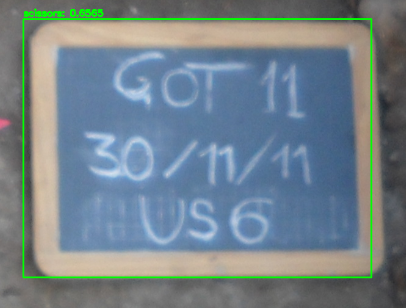
\includegraphics[width =0.5\textwidth]{scissors.PNG}
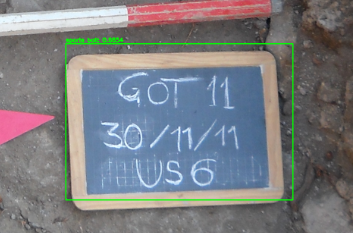
\includegraphics[width =0.5\textwidth]{sportsball.PNG}
\caption{Erkennung und Kategorisierung der Tafeln als Schere oder Sportball.}
\label{fig:cnnboard}
\end{figure}

%Adaptiver Ansatz: 292 Bilder input, 133 output, davon 8 Fp und 0 FN, Rest dementsprechend TP. recall = 1, precision = 0.926, f = 0.961 -> Mehr TP als Bilder mit Tafeln, bedingt durch das Verfahren, Einfluss auf statistische Auswertung aber gering
%Iterativer Ansatz: 292 Bilder input, 85 output, davon 6 fp und 0 fn. recall =1, precision = 0.929, f = 0.963
%Fehler vor allem durch Bild mit Plakat. Ohne diese Bilder (1081,1082,1083,1084):
%Adaptiver Ansatz: 292 Bilder input, 127 output, davon 2 Fp und 0 FN, Rest dementsprechend TP. recall = 1, precision = 0.984, f = 0.992
%Iterativer Ansatz: 292 Bilder input, 81 output, davon 2 fp und 0 fn. recall =1, precision = 0.975, f = 0.987
%-> Adaptiver Ansatz insgesamt etwas besser, iterativer etwas robuster, insgesamt aber Unterschiede zu vernachlässigen

%Tafelrkennung: Unterschied zwischen adpativem und iterativen Threshold
Bei der Auswertung der Texterkennung nach Detektionsverfahren ergaben sich Unterschiede: Beim adaptiven Verfahren (ausgewertet mit beiden Schnittverfahren) lag der \textit{F-Score} der \textit{Endauswahl} bei 0.59, das theoretische Optimum bei 0.67 (Vgl. adaptive only.csv). Das iterative Verfahren kam auf einen \textit{F-Score} von 0.56 bei einem Optimum von 0.65 (Vgl. iterative only.csv).
%Tafelerkennung: Unterschied zwischen simple und hough crop
Beim nächsten Schritt, dem Schnittverfahren, variierten die Ergebnisse deutlicher. So erzielte die  \textit{Endauswahl} des \verb|Hough Crop|-Verfahrens (iterativer und adaptiver Ansatz parallel) einen \textit{F-Score} von 0.49, das theoretische Optimum betrug 0.59 (Vgl. hough only.csv). Im Gegensatz dazu lag die \textit{Endauswahl} des \verb|Simple Crop| bei 0.62 und somit noch über der Gesamtauswertung. Das theoretische Optimum lag mit 0.67 etwas unter der Gesamtauswertung (Vgl. simple only.csv).
Als Einzelverfahren war die Kombination \verb|Adaptive Simple Crop| am besten, mit einem \textit{Gesamt}-Durchschnitt von 0.61 und einem theoretischen Optimum von 0.64 (Vgl. crop adaptive simple.csv).\\
\\
\begin{table}
\begin{tabular}[h!]{c|c|c|c|c|c}
Verfahren & Buchstaben & Zeilen & Gesamt & Endauswahl & Optimum \\
\hline
Gesamt & 0.47 & 0.51 & 0.49 & 0.61 & 0.7 \\
Adaptive (Hough + Simple) & 0.47 & 0.51 & 0.49 & 0.59 & 0.67\\
Iterative (Hough + Simple) & 0.48 & 0.51 & 0.5 & 0.56 & 0.65\\
Hough (Adaptive + Iterative) & 0.43 & 0.47 & 0.45 & 0.49 & 0.59\\
Simple (Adaptive + Iterative) & 0.52 & 0.56 & 0.54 & 0.62 & 0.67\\
\end{tabular}
\caption{\label{tab:Tabelle2}Mittelwerte der Ergebnisse bei der Anwendung aller Verfahren gleichzeitig sowie der beiden Detektionsverfahren und der beiden Schnittverfahren untereinander. Angegeben sind die F-Werte für das \textbf{Buchstaben}verfahren (image to box), das \textbf{Zeilen}verfahren (image to text), der \textbf{Gesamt}durchschnitt beider Verfahren, die durch den Algorithmus vorgenommene \textbf{Endauswahl} sowie das theoretische \textbf{Optimum}, also die tatsächliche beste Auswahl.}
\end{table} 
%Tafelerkennung: Cont based cut? -> Diskussion
%Tafelerkennung: Ausfilterung der hough crop-Bilder mit Rahmen im Bild -> besseres Ergebnis?


\subsection{Texterkennung}
%Texterkennung: Unterschied zwischen Box und Text
Im Bereich der Texterkennung ließ sich ein Unterschied zwischen \verb|Image to Box|, also der Buchstabenerkennung, und \verb|Image to Text|, der Zeilenerkennung, feststellen. So war der mittlere \textit{F-Score} bei der Buchstabenerkennung um 0.03 bis 0.05 niedriger als bei der Zeilenerkennung (Vgl. collection.csv u.a.). Im Einzelfall variierten die Ergebnisse jedoch stark, sodass die Buchstabenerkennung deutlich bessere Ergebnisse als die Zeilenerkennung liefern kann, was sich positiv auf den \textit{bestguess} auswirkt.
%Texterkennung: Unterschied zwischen Dictioniary und ohne Dictionary
%Texterkennung: Unterschied zwischen Whitelist und ohne Whitelist
Wie bereits vorgestellt wurde für die Texterkennung ein Wörterbuch und eine Whitelist verwendet. In der Auswertung zeigte sich, dass vor allem die Whitelist das Ergebnis deutlich verbessert. Die Anwendung der Texterkennung ohne Wörterbuch, aber mit Whitelist, auf die mit \verb|Adaptive Simple Crop| erzeugten Tafelausschnitte erzielte die gleichen Ergebnisse wie der Durchlauf mit Wörterbuch, also einen Durchschnitt von 0.61 bei der \textit{Endauswahl}(Vgl. no dic.csv). Wurden sowohl Whitelist als auch Wörterbuch entfernt, sank der durchschnittliche \textit{F-Score} auf 0.26, wobei die Buchstabenerkennung 0.25 erzielte, die Zeilenerkennung nur 0.01 (Vgl. no config no dic.csv). Schaltete man nur das Wörterbuch dazu, verbesserte sich der Wert der Zeilenerkennung auf 0.26 (Vgl. dic only.csv).
%Bestguess erklären und auswerten
%Problem der theroetisch noch höheren Genauigkeit ansprechen (Auswahl durch Länge ungenügend)
Festzustellen war auch, dass die \textit{Endauswahl} nicht zu Ergebnissen unterhalb es Durchschnitts führte, andererseits aber für deutliche Verbesserungen sorgen konnte. Deutlich wurde das in der Gesamtauswertung aller Ansätze, bei der die Differenz zwischen dem durchschnittlichen \textit{F-Score} der beiden Texterkennungsverfahren (0.49) und dem durchschnittlichen \textit{F-Score} der \textit{Endauswahl}(0.61) 0.12 Punkte betrug. Allerdings bestand auch ein Unterschied von 0.9 zum theoretischen Optimum (0.7) (Vgl. collection.csv).

% Anwendung auf neue Tafeln

\subsection{Weitere Tafeln}

Bei der Anwendung des Algorithmus auf die projektfremden Tafeln der Gruppe Terrestrische Ökohydrologie der FSU Jena sowie der späteren Grabungen am Kapitol durch das Deutsche Archäologische Institut ergaben sich folgende Ergebnisse:
Bei den Tafeln der Ökohydrologie Jena wurde eine Stichprobe aus 40 Fotos mit Tafeln verwendet. Von diesen wurden 9 korrekt erkannt. Auf 16 Fotos wurde fälschlicherweise ein beiliegendes Maßband erkannt\footnote{Hier ist technisch gesehen kein unerwünschtes Ergebnis erzielt worden: Auch das Maßband enthält rechteckige Felder mit passendem Seitenverhältnis und Zahlen darauf.}. Der \textit{Recall} beträgt hier 0.225, die \textit{Precision} 0.36. Der \textit{F-Score} liegt bei 0.277. Diese Ergebnisse wurden mit dem iterativen Verfahren erzielt. Mittels adaptivem Ansatz konnten keine Tafeln ermittelt werden. Die Texterkennung verlief -- abgesehen von Zahlen auf dem Maßband -- ergebnislos.
Aus den Fotografien der Grabungen des DAI wurden 35 Bilder mit Tafeln darauf ausgewählt. Mit dem adaptiven Verfahren wurden 26 Tafeln erkannt, dazu gab es eine Falsch-Positive. Daraus ergab sich ein \textit{Recall} von 0.743, eine \textit{Precision} von 0.963 und ein {F-Score} von 0.838. Das iterative Verfahren erkannte 25 Tafeln ohne Falsch-Positive. Der \textit{Recall} betrug hier 0.714, die \textit{Precision} 1 und der \textit{F-Score} 0.833.
Für die Texterkennung wurde die Whitelist modifiziert, sodass alle Ziffern und alle Großbuchstaben enthalten waren, wie es der Beschriftung der Tafeln entspricht. Der \textit{F-Score} der Zeilenerkennung lag bei 0.86, der der Buchstabenerkennung bei 0.9. Das theoretische Optimum lag bei 0.91. Der \textit{bestguess} lag mit 0.83 deutlich unter diesen Werten. Ohne Whitelist konnten lediglich Werte von 0.04 bei der Zeilenerkennung, bzw. 0.64 bei der Buchstabenerkennung erzielt werden.
